%%%%%%%%%%%%%%%%%%%%%%%%%%%%%%%%%%%%%%%%%%%%%%%%%%%%%%%%%%%%%%%%%%%%%%%%
%                                                                      %
%     File: IST_Report_Architecture.tex                                    %
%                                                                      %
%%%%%%%%%%%%%%%%%%%%%%%%%%%%%%%%%%%%%%%%%%%%%%%%%%%%%%%%%%%%%%%%%%%%%%%%
% !TEX root = IST_Report.tex
\clearpage

\chapter{Arquitectura}
\label{chapter:architecture}
Neste capítulo é apresentada a arquitectura do sistema, a interligação entre os vários módulos e uma explicação  detalhada do funcionamento dos vários procedimentos como a cifra e assinatura.
% ----------------------------------------------------------------------
\section{Visão Geral}
\label{section:estrutura}
A solução desenvolvida permite a troca de mensagens de modo seguro e com garantias temporais. Esta solução é constituída por 3 módulos: Sender, Receiver e um servidor de Timestamp (\textbf{Figura~\ref{fig:chart}}).\\

\begin{figure}[htp]
\centering 
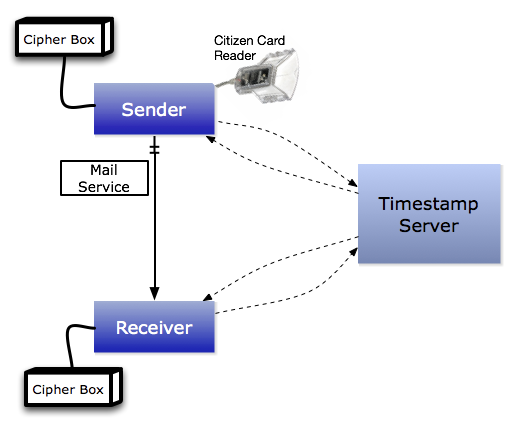
\includegraphics[width=12cm]{./Figures/chart.png}
\caption{Arquitectura do Sistema}
\label{fig:chart}
\end{figure}

O Sender pretende enviar um conjunto de dados para o receiver mas com garantias de \textbf{confidencialidade}, \textbf{autenticidade}, \textbf{não repudiação} e instante temporal. Estas garantias são dadas por mecanismos externos: CipherBox, Cartão Cidadão e Servidor Timestamp, respectivamente.\\

Num cenário de utilização, o sender selecciona a pasta que pretende enviar e escolhe cada uma das seguintes acções:
\begin{itemize}
\item Sign - assinar o(s) ficheiro(s) com o seu Cartão de Cidadão da República Portuguesa
\item Timestamp - adicionar um timestamp seguro assinado por uma Autoridade Certificada
\item Cipher - cifrar o(s) ficheiro(s)
\end{itemize}

Supondo que todas as opções foram seleccionadas é realizada a cadeia de acções descrita na \textbf{Figura~\ref{fig:order}}. \\

\begin{figure}[htp]
\centering 
\includegraphics[width=8cm]{./Figures/Architecture.pdf}
\caption{Ordem de execução}
\label{fig:order}
\end{figure}

Os ficheiros seleccionados, são comprimidos num único. De seguida este ficheiro é assinado recorrendo ao Cartão de Cidadão e o seu \textit{hash} é enviado ao servidor de timestamp seguro. O servidor cria um par associando um instante temporal ao hash. Este par é assinado pelo servidor afim de garantir que o servidor recebeu o hash naquele instante. Este certificado de Timestamp é devolvido ao sender.\\ 
A assinatura de cartão de cidadão, o certificado de Timestamp e os dados são organizados numa estrutura e esta estrutura é cifrada. Os dados cifrados são colocados dentro de uma nova estrutura que descreve as operações realizadas e permite inverter o processo. A estrutura é então codificada e escrita em disco em formato de ficheiro para que o Sender possa enviar. \\
 
Quando o Receiver recebe este ficheiro protegido efectua as operações pela ordem inversa, começando pela decifra, verificação da validade do Timestamp através do servidor, verificação a Assinatura e descomprimindo os dados.

\section{Zipping/Unzipping}
Sempre que o Sender envia uma mensagem, seleciona a pasta que pretende enviar. Esta pasta é comprimida utilizando a biblioteca \textit{Zip} nativa do Java 6. O output desta operação é um ficheiro único que contém toda a pasta comprimida e por isso reduz a dimensão do anexo a cifrar, assinar e enviar.\\
É então criada uma estrutura que será preenchida nos próximos passos com os metadados.
\section{Sign/Verify}
A segunda operação a ser executada pelo Sender é a operação de Assinatura; no caso do Receiver esta é a penultima última operação a ser executada (antes do unzip). \\
Para garantir a não repudiação e autenticidade do ficheiro comprimido é utilizado o Cartão do Cidadão através da biblioteca PKCS11. O ficheiro é \textit{hashed} com SHA-1 e assinados pela chave RSA privada contida no cartão de cidadão. A assinatura e o Certificado de chave pública do cartão de cidadão são colocados na estrutura de metadados. \\

Do lado do Receiver, a assinatura é verificada em 2 passos. Primeiro verificamos se o certificado enviado é válido, verificando a assinatura do certificado contra os \textit{root certificate} do Estado Português que é incluído na solução. De seguida, verifica se a mensagem foi assinada pelo detentor do certificado. Caso a mensagem seja válida, é apresentado o nome do detentor do certificado.\\
Este mecanismo possui uma optimização por assinar apenas o contéudo comprimido. Não obstante,\textbf{ garantimos apenas a não repudiação do contéudo comprimido e não do contéudo original.} 

\section{Timestamp Seguro}
\label{section:timestamp}
Para utilizar um mecanismo de Timestamp seguro, o Sender envia ao Servidor de Timestamp um pedido com o hash do(s) ficheiro(s).\\
 O servicor cria um Timestamp com a data actual e anexa-o ao hash recebido. Este par é assinado com a chave privada do servidor, criando uma mensagem com o formato: \textit{Kp(H(m),T),T}
Em que H(m) é a hash da mensagem, T o timestamp e Kp a chave privada do Servidor de Timestamp. \\
Este serviço apenas garante que \textbf{este hash foi assinado pelo servidor na data definida.} \\

O Receiver verifica a validade do timestamp, ou seja, o momento em que o servidor de confiança associou o hash da mensagem. Para tal, é utilizado o certificado do Servidor de Timestamp seguro que está incluido no pacote da solução. \\
Não é dada qualquer garantia da data de envio de email porque o utilizador pode enviar o mail à-posteriori. \\

\section{Cipher/Decipher}
A última operação a ser executada pelo Sender e a primeira a ser executada pelo Receiver é a operação de cifra (e decifra, respectivamente).
Para efectuar a cifra, o Sender utiliza a Caixa de Cifra via ethernet fornecida pelo Cliente. O software base para connecção com a caixa foi disponibilizado em C. As invocações Java foram convertidas para invocações C através do JNI.
A mensagem é cifrada por blocos, o que possibilita a cifra de ficheiros de grandes dimensões.
O Receiver utiliza também uma Caixa de Cifra ethernet para decifrar a mensagem.\\
Esta caixa realiza cifra e decifra AES. A chave utilizada está contida na caixa por isso esta caixa constitui um mecanismo de segredo partilhado, ou seja, apenas quem tem a caixa pode decifrar o contéudo.

\section{Base64}
Antes de salvar (ou enviar para o email) o ficheiro gerado é codificado em base64. Este sistema codifica cada byte em 6 bits. Estes 6 bits são caracteres conhecidos pela norma ASCII e por isso o ficheiro pode ser enviado em formato de \textit{plain-text} sem que alguns sistemas de codificação e \textit{sanitize} removam caracteres desconhecidos e deste modo adulterem o contéudo da mensagem.


